\documentclass[]{article}
\usepackage{lmodern}
\usepackage{amssymb,amsmath}
\usepackage{ifxetex,ifluatex}
\usepackage{fixltx2e} % provides \textsubscript
\ifnum 0\ifxetex 1\fi\ifluatex 1\fi=0 % if pdftex
  \usepackage[T1]{fontenc}
  \usepackage[utf8]{inputenc}
\else % if luatex or xelatex
  \ifxetex
    \usepackage{mathspec}
    \usepackage{xltxtra,xunicode}
  \else
    \usepackage{fontspec}
  \fi
  \defaultfontfeatures{Mapping=tex-text,Scale=MatchLowercase}
  \newcommand{\euro}{€}
\fi
% use upquote if available, for straight quotes in verbatim environments
\IfFileExists{upquote.sty}{\usepackage{upquote}}{}
% use microtype if available
\IfFileExists{microtype.sty}{%
\usepackage{microtype}
\UseMicrotypeSet[protrusion]{basicmath} % disable protrusion for tt fonts
}{}
\usepackage[margin=1in]{geometry}
\usepackage{color}
\usepackage{fancyvrb}
\newcommand{\VerbBar}{|}
\newcommand{\VERB}{\Verb[commandchars=\\\{\}]}
\DefineVerbatimEnvironment{Highlighting}{Verbatim}{commandchars=\\\{\}}
% Add ',fontsize=\small' for more characters per line
\usepackage{framed}
\definecolor{shadecolor}{RGB}{248,248,248}
\newenvironment{Shaded}{\begin{snugshade}}{\end{snugshade}}
\newcommand{\KeywordTok}[1]{\textcolor[rgb]{0.13,0.29,0.53}{\textbf{{#1}}}}
\newcommand{\DataTypeTok}[1]{\textcolor[rgb]{0.13,0.29,0.53}{{#1}}}
\newcommand{\DecValTok}[1]{\textcolor[rgb]{0.00,0.00,0.81}{{#1}}}
\newcommand{\BaseNTok}[1]{\textcolor[rgb]{0.00,0.00,0.81}{{#1}}}
\newcommand{\FloatTok}[1]{\textcolor[rgb]{0.00,0.00,0.81}{{#1}}}
\newcommand{\CharTok}[1]{\textcolor[rgb]{0.31,0.60,0.02}{{#1}}}
\newcommand{\StringTok}[1]{\textcolor[rgb]{0.31,0.60,0.02}{{#1}}}
\newcommand{\CommentTok}[1]{\textcolor[rgb]{0.56,0.35,0.01}{\textit{{#1}}}}
\newcommand{\OtherTok}[1]{\textcolor[rgb]{0.56,0.35,0.01}{{#1}}}
\newcommand{\AlertTok}[1]{\textcolor[rgb]{0.94,0.16,0.16}{{#1}}}
\newcommand{\FunctionTok}[1]{\textcolor[rgb]{0.00,0.00,0.00}{{#1}}}
\newcommand{\RegionMarkerTok}[1]{{#1}}
\newcommand{\ErrorTok}[1]{\textbf{{#1}}}
\newcommand{\NormalTok}[1]{{#1}}
\usepackage{graphicx}
\makeatletter
\def\maxwidth{\ifdim\Gin@nat@width>\linewidth\linewidth\else\Gin@nat@width\fi}
\def\maxheight{\ifdim\Gin@nat@height>\textheight\textheight\else\Gin@nat@height\fi}
\makeatother
% Scale images if necessary, so that they will not overflow the page
% margins by default, and it is still possible to overwrite the defaults
% using explicit options in \includegraphics[width, height, ...]{}
\setkeys{Gin}{width=\maxwidth,height=\maxheight,keepaspectratio}
\ifxetex
  \usepackage[setpagesize=false, % page size defined by xetex
              unicode=false, % unicode breaks when used with xetex
              xetex]{hyperref}
\else
  \usepackage[unicode=true]{hyperref}
\fi
\hypersetup{breaklinks=true,
            bookmarks=true,
            pdfauthor={Aaron Augustine},
            pdftitle={Is Transmission type better for MPG},
            colorlinks=true,
            citecolor=blue,
            urlcolor=blue,
            linkcolor=magenta,
            pdfborder={0 0 0}}
\urlstyle{same}  % don't use monospace font for urls
\setlength{\parindent}{0pt}
\setlength{\parskip}{6pt plus 2pt minus 1pt}
\setlength{\emergencystretch}{3em}  % prevent overfull lines
\setcounter{secnumdepth}{0}

%%% Use protect on footnotes to avoid problems with footnotes in titles
\let\rmarkdownfootnote\footnote%
\def\footnote{\protect\rmarkdownfootnote}

%%% Change title format to be more compact
\usepackage{titling}

% Create subtitle command for use in maketitle
\newcommand{\subtitle}[1]{
  \posttitle{
    \begin{center}\large#1\end{center}
    }
}

\setlength{\droptitle}{-2em}
  \title{Is Transmission type better for MPG}
  \pretitle{\vspace{\droptitle}\centering\huge}
  \posttitle{\par}
  \author{Aaron Augustine}
  \preauthor{\centering\large\emph}
  \postauthor{\par}
  \predate{\centering\large\emph}
  \postdate{\par}
  \date{August 11, 2015}



\begin{document}

\maketitle


\section{Executive Summary}\label{executive-summary}

The purpose of this paper is to explore the relationship between a set
of variables and miles per gallon(mpg) as part of a class project using
the mtcars dataset. It will focus on answering two questions: ``Is an
automatic or manual transmission better for MPG'' and ``Quantify the MPG
difference between automatic and manual transmissions''. Based on the
analysis below there is a relationsip between MPG and transmission type.

\section{Data Analysis}\label{data-analysis}

\subsection{EDA}\label{eda}

First we'll start by exploring relationships in the data. We'll do this
by creating a correlation matrix and pairwise plots of all of the
variabes. (See appendix). Interestingly enough all the variables seem to
have strong correlations with mpg. It's also noted that we will need to
convert several of the variables from numeric to factor variables prior
to feeding into a regression model.

From there we will work to build a regression model to determine
determine how Transmission (0 = automatic, 1 = manual) relates to MPG.

\subsection{Variable Selection and model
building}\label{variable-selection-and-model-building}

To get started with variable selection we start with a simple model of
transmission vs.~mpg.

\begin{Shaded}
\begin{Highlighting}[]
\NormalTok{fit1 <-}\StringTok{ }\KeywordTok{lm}\NormalTok{(mpg~am,}\DataTypeTok{data=}\NormalTok{regdata)}
\end{Highlighting}
\end{Shaded}

The model is significant with a p-value of 0.000285020744. However,
given the lower R-squared 0.33846 we'll work to include more predictors
to get a better explaination of the variable in mpg. To do this we'll
run a stepwise regression and compare the models.

\begin{Shaded}
\begin{Highlighting}[]
\NormalTok{fit2 <-}\StringTok{ }\KeywordTok{lm}\NormalTok{(mpg~cyl+disp+hp+drat+wt+qsec+vs+am+gear+carb,}\DataTypeTok{data=}\NormalTok{regdata)}
\NormalTok{stepModel <-}\StringTok{ }\KeywordTok{step}\NormalTok{(fit2, }\DataTypeTok{k=}\KeywordTok{log}\NormalTok{(}\KeywordTok{nrow}\NormalTok{(regdata)))}
\end{Highlighting}
\end{Shaded}

From the stepwise regression, we find a signifcant model with a pvalue
of 1.2e-11 and a much better R-squared, 0.83356.

Comparing the two models using the anova function we also verify that
adding in wt and qsec is than just am.

\begin{Shaded}
\begin{Highlighting}[]
\KeywordTok{anova}\NormalTok{(fit1,stepModel)}
\end{Highlighting}
\end{Shaded}

\begin{verbatim}
## Analysis of Variance Table
## 
## Model 1: mpg ~ am
## Model 2: mpg ~ wt + qsec + am
##   Res.Df RSS Df Sum of Sq    F  Pr(>F)    
## 1     30 721                              
## 2     28 169  2       552 45.6 1.6e-09 ***
## ---
## Signif. codes:  0 '***' 0.001 '**' 0.01 '*' 0.05 '.' 0.1 ' ' 1
\end{verbatim}

With a model selected lets do some quick diagnostic plots.

\begin{Shaded}
\begin{Highlighting}[]
\KeywordTok{par}\NormalTok{(}\DataTypeTok{mfrow=}\KeywordTok{c}\NormalTok{(}\DecValTok{2}\NormalTok{,}\DecValTok{2}\NormalTok{))}
\KeywordTok{plot}\NormalTok{(stepModel)}
\end{Highlighting}
\end{Shaded}

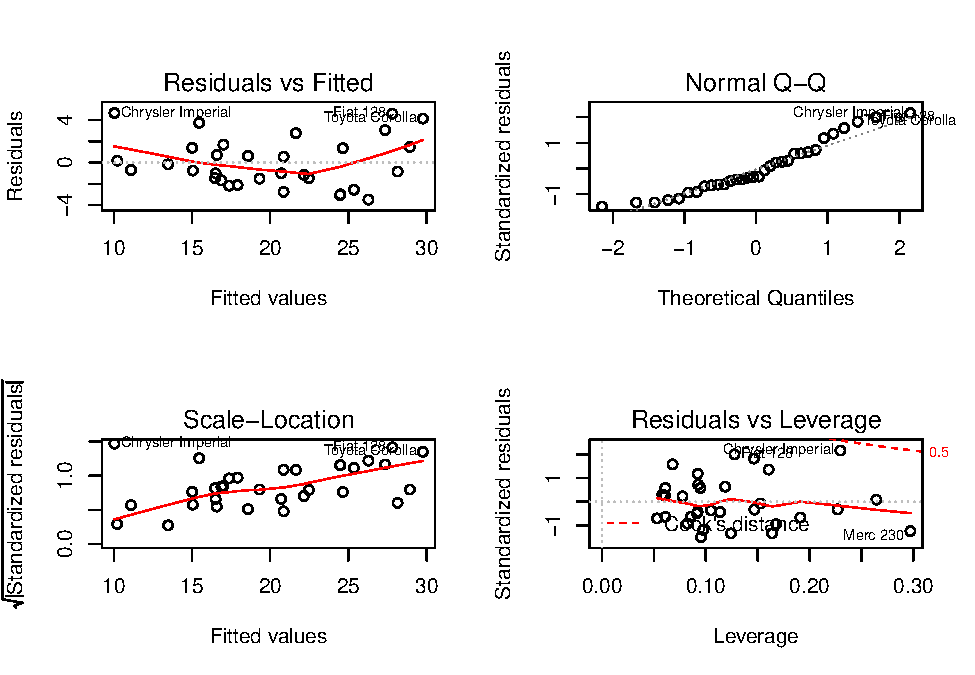
\includegraphics{statproject_files/figure-latex/unnamed-chunk-6-1.pdf}

Looking at the plot of the fit values vs.~the residuals, there does not
seem to be any heteroskedasticity and the errors center around zero. The
Normal Q-Q plot also doesn't show any strong depatures from normality.
The Scale Location and Residuals vs.~Leverage

Lastly, to answer the given questions, we can execute a T-test on the
transition parameter,am, from the model. From this we can find that the
paramater is moderately signifcant, 0.04672. Thus, a manual transmission
provides 2.93584 more miles per gallon keeping in mind there is a lot
variation around the estimate. The 95\% CI for the interval is
{[}0.04573,5.82594{]}.

\section{Appendix}\label{appendix}

Plots

\begin{Shaded}
\begin{Highlighting}[]
\KeywordTok{head}\NormalTok{(mtcars)}
\end{Highlighting}
\end{Shaded}

\begin{verbatim}
##                    mpg cyl disp  hp drat    wt  qsec vs am gear carb
## Mazda RX4         21.0   6  160 110 3.90 2.620 16.46  0  1    4    4
## Mazda RX4 Wag     21.0   6  160 110 3.90 2.875 17.02  0  1    4    4
## Datsun 710        22.8   4  108  93 3.85 2.320 18.61  1  1    4    1
## Hornet 4 Drive    21.4   6  258 110 3.08 3.215 19.44  1  0    3    1
## Hornet Sportabout 18.7   8  360 175 3.15 3.440 17.02  0  0    3    2
## Valiant           18.1   6  225 105 2.76 3.460 20.22  1  0    3    1
\end{verbatim}

\begin{Shaded}
\begin{Highlighting}[]
\KeywordTok{str}\NormalTok{(mtcars)}
\end{Highlighting}
\end{Shaded}

\begin{verbatim}
## 'data.frame':    32 obs. of  11 variables:
##  $ mpg : num  21 21 22.8 21.4 18.7 18.1 14.3 24.4 22.8 19.2 ...
##  $ cyl : num  6 6 4 6 8 6 8 4 4 6 ...
##  $ disp: num  160 160 108 258 360 ...
##  $ hp  : num  110 110 93 110 175 105 245 62 95 123 ...
##  $ drat: num  3.9 3.9 3.85 3.08 3.15 2.76 3.21 3.69 3.92 3.92 ...
##  $ wt  : num  2.62 2.88 2.32 3.21 3.44 ...
##  $ qsec: num  16.5 17 18.6 19.4 17 ...
##  $ vs  : num  0 0 1 1 0 1 0 1 1 1 ...
##  $ am  : num  1 1 1 0 0 0 0 0 0 0 ...
##  $ gear: num  4 4 4 3 3 3 3 4 4 4 ...
##  $ carb: num  4 4 1 1 2 1 4 2 2 4 ...
\end{verbatim}

\begin{Shaded}
\begin{Highlighting}[]
\KeywordTok{cor}\NormalTok{(mtcars)}
\end{Highlighting}
\end{Shaded}

\begin{verbatim}
##           mpg      cyl     disp       hp      drat       wt      qsec
## mpg   1.00000 -0.85216 -0.84755 -0.77617  0.681172 -0.86766  0.418684
## cyl  -0.85216  1.00000  0.90203  0.83245 -0.699938  0.78250 -0.591242
## disp -0.84755  0.90203  1.00000  0.79095 -0.710214  0.88798 -0.433698
## hp   -0.77617  0.83245  0.79095  1.00000 -0.448759  0.65875 -0.708223
## drat  0.68117 -0.69994 -0.71021 -0.44876  1.000000 -0.71244  0.091205
## wt   -0.86766  0.78250  0.88798  0.65875 -0.712441  1.00000 -0.174716
## qsec  0.41868 -0.59124 -0.43370 -0.70822  0.091205 -0.17472  1.000000
## vs    0.66404 -0.81081 -0.71042 -0.72310  0.440278 -0.55492  0.744535
## am    0.59983 -0.52261 -0.59123 -0.24320  0.712711 -0.69250 -0.229861
## gear  0.48028 -0.49269 -0.55557 -0.12570  0.699610 -0.58329 -0.212682
## carb -0.55093  0.52699  0.39498  0.74981 -0.090790  0.42761 -0.656249
##            vs        am     gear      carb
## mpg   0.66404  0.599832  0.48028 -0.550925
## cyl  -0.81081 -0.522607 -0.49269  0.526988
## disp -0.71042 -0.591227 -0.55557  0.394977
## hp   -0.72310 -0.243204 -0.12570  0.749812
## drat  0.44028  0.712711  0.69961 -0.090790
## wt   -0.55492 -0.692495 -0.58329  0.427606
## qsec  0.74454 -0.229861 -0.21268 -0.656249
## vs    1.00000  0.168345  0.20602 -0.569607
## am    0.16835  1.000000  0.79406  0.057534
## gear  0.20602  0.794059  1.00000  0.274073
## carb -0.56961  0.057534  0.27407  1.000000
\end{verbatim}

\begin{Shaded}
\begin{Highlighting}[]
\KeywordTok{pairs}\NormalTok{(mtcars, }\DataTypeTok{panel=}\NormalTok{panel.smooth)}
\end{Highlighting}
\end{Shaded}

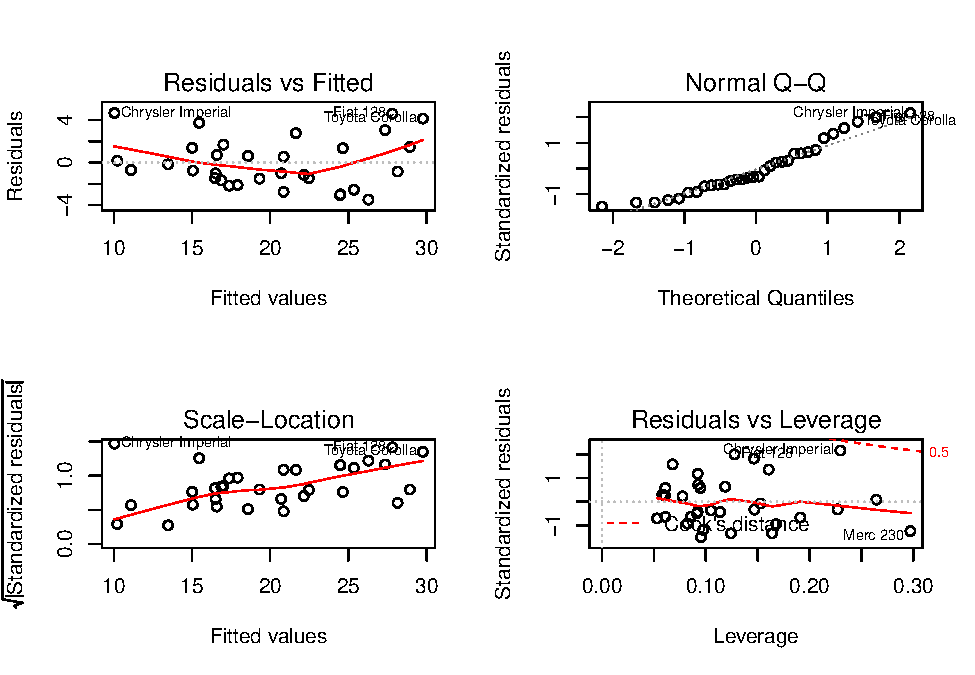
\includegraphics{statproject_files/figure-latex/unnamed-chunk-7-1.pdf}

\end{document}
